\documentclass[a4paper,12pt]{article}
% packages and main settings
\usepackage[left=3cm, right=2cm, top=2cm, bottom=2cm]{geometry}
\usepackage[english]{babel}    
\usepackage[utf8]{inputenc}  
\usepackage[T1]{fontenc}        
\usepackage{lmodern}            
\usepackage{microtype}          
\usepackage{amsmath}
\usepackage{amsfonts, amsthm, amssymb, graphicx, booktabs}
\usepackage{newclude}   
\usepackage{placeins}  %surpresses floating tables
\usepackage[labelfont=sc]{caption} %Figure etc steht dann in small caps 
\usepackage[flushleft]{threeparttable} % for notes below table
\usepackage{multirow} % for table cell merge along rows
\usepackage{graphicx} % to adjust tablesize to textwidth
\usepackage{caption}  % for centered captions
\usepackage{float} % to set of autopositioning of tables
\usepackage[bottom]{footmisc} % forces footnotes to the bottom
\usepackage{setspace}           % Fuer 1.5 fachen Zeilenabstand  
\onehalfspacing % 1.5 cm Zeilenabstand
%Bibtex
\usepackage[round]{natbib}
\bibliographystyle{chicago} % chicago bib style like in AER
\usepackage[hidelinks]{hyperref} % fuer links und verweise. Cleverref ist eigentlich besser. 


% Create header. The header must be surpressed for 
% every first page per section and a solution
% for the Appendix is used in the respective subfile.
\usepackage{fancyhdr}
\pagestyle{fancy}
\fancyhf{}
\chead{\nouppercase{\textit{\leftmark}}}
\cfoot{\thepage}
\renewcommand{\headrulewidth}{0pt} % no vertical line

%\usepackage{lipsum}  % check if formats work

\usepackage{afterpage} %clearpage w/o pagebreak for "header bug"

% Expectation symbol
\DeclareMathOperator*{\E}{\mathbb{E}}


% for more space in tables
%\usepackage[landscape]{geometry}% http://ctan.org/pkg/geometry
%\usepackage{array}% http://ctan.org/pkg/array

% for gray table row color
\usepackage[table]{xcolor}

% decimal dot alignment in table columns
\usepackage{siunitx}

% for footnotes in table
\usepackage[flushleft]{threeparttable}


\usepackage{tikz}
\begin{document}

\section{Model and Parametrization}
\thispagestyle{plain} % surpress header on first page
This section introduces the economic model to which the UQ is applied. It is the dynamic model of occupational choice developed in \cite{Keane.1994}. [Add further remarks on its relevance and \cite{Keane.1997}.] First, I outline the general choice-theoretic framework and the concrete specification of the model. This includes the set of uncertain model parameters. Then, I present the approach that  \citeauthor{Keane.1997} use to estimate these model parameters given data on occupational choices. After that, their results for the means and variances of the respective estimates are shown. These constitute the parametrization for the input distribution in the UQ. The section continues with remarks on the numerical implementation. It concludes with the presentation of the QoI.


\subsection{Economic Model}

\cite{Keane.1994} develop a dynamic economic model to explain occupation decisions between compulsory schooling and pension age. In the general choice-theoretic framework, a representative agent decides for occupation $m$ between $M$ alternatives at each age $a \in A$. These alternatives are mutually exclusive. The decision for occupation $m'$ at age $a$ is denoted by $d_{m'}(a)=1$. This equation is equivalent to $d_{m \in M\setminus m'}(a)=0$. Each occupation decision is immediately rewarded by $R_m(S(a))$. Partly, rewards and prior decisions are intertemporally connected: Agents receive higher rewards if they accumulated skills in past occupations that are useful for the present one. $S(a)$ denotes the state space. The state space is the set of information at age $a$ relevant for the present and future rewards for each occupation choice. $R_m$ is subject to random shocks. The flow of events is depicted in Figure X. \\

\begin{figure}[H]
\caption{Flow of events}
\vspace{-0.0cm}

	\begin{center}
		
		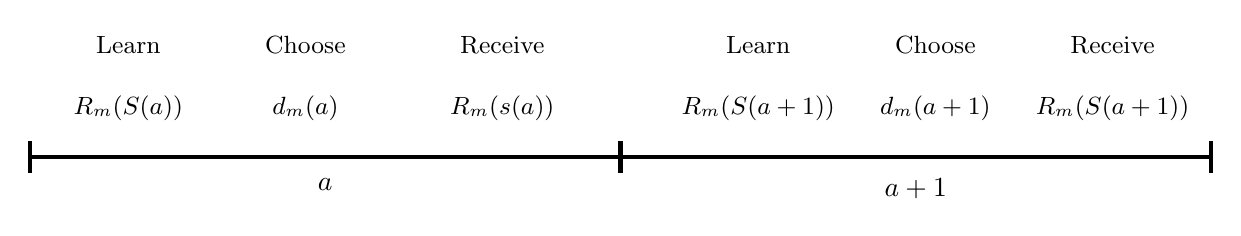
\begin{tikzpicture}
		\draw [ultra thick] (0,0) -- (15,0);
		\foreach \x in {0,7.5,15}
		\draw [ultra thick] (\x cm,0.2) -- (\x cm, -0.2);
		\small % derease fontsize
		\draw (1.25,0) node[above=0.35cm] {$R_m(S(a))$};
		\draw (3.50,0) node[above=0.35cm] {$d_m(a)$};
		\draw (6.0,0) node[above=0.35cm] {$R_m(s(a))$};
		\draw (9.25,0) node[above=0.35cm] {$R_m(S(a+1))$};
		\draw (11.5,0) node[above=0.35cm] {$d_m(a+1)$};
		\draw (13.75,0) node[above=0.35cm] {$R_m(S(a+1))$};
		
		\draw (1.25,0) node[above=1.2cm] {Learn};
		\draw (3.50,0) node[above=1.2cm] {Choose};
		\draw (6.0,0) node[above=1.2cm] {Receive};
		\draw (9.25,0) node[above=1.2cm] {Learn};
		\draw (11.5,0) node[above=1.2cm] {Choose};
		\draw (13.75,0) node[above=1.2cm] {Receive};
		
		\normalsize %reincrease fontsize
		\draw (3.75,0) node[below=0.15cm] {$a$};
		\draw (11.25,0) node[below=0.15cm] {$a+1$};
		%\draw (2.35,0) node[above=6pt, align=center] {(estimation \\ window]};
		\end{tikzpicture}
	\end{center}
\end{figure}



\noindent
At the beginning of each age $a$, the agent recognizes the reward shocks, and the shocks become part of the state space. Thus, $R_m(S(a))$ is known to the agent at age $a$. However, he can only form expectations about rewards in the future. Given \citeauthor{Keane.1994}'s concrete specification, it is assumed that shocks to the reward function are not serially correlated. Therefore, prior shocks do not enter the state space. Thus, the state space comprises the history of choices or, in other words, the occupation experience and the realizations of the contemporaneous shocks. Next, the agent chooses his occupation based on state space information. Then he receives the occupation-specific reward. This flow repeats for each $a < A$.

Agents are rational and forward-looking. Future rewards are subject to time discount factor $\delta  \in [0,1]$. Hence, they choose their optimal sequence of occupations by maximizing the \textit{remaining} expected, discounted life-time rewards \textit{at each age}. This maximal value is given by the value function $V(S(a),a)$.
 
\begin{align}
V(S(a),a) = \max_{(d_m(a))_{m \epsilon M}} \E\bigg[\sum_{\tau=a}^T \delta^{\tau-a} \sum_{m=1}^M R_m(a)d_m(a) | S(a)\bigg]
\end{align}
Value $V$ depends directly on age $a$ because $A$ is finite. To re-write the maximization problem as Bellman equation (\cite{Bellman.1957}; rquation \ref{eq:Bellman_b}), it is noted that the value function equals the maximal choice-specific value function (equation \ref{eq:Bellman_a}).

\begin{align} \label{eq:Bellman_a}
V(S(a),a) = \max_{m \epsilon M} V_m(S(a),a)
\end{align}

\begin{align} \label{eq:Bellman_b}
V_m(S(a),a) = \max_{d_m(a)} \bigg\{R_m(S(a),a) + \delta \E\big[V(S(a+1),a+1)\big] \bigg\}
\end{align}
Taken together, the above two equations constitute the dynamic programming problem for the general choice-theoretic framework. The agent computes his potential return for every possible scenario order to make the optimal decision. Therefore, this problem is solved for every point in the state space.

The economic model of occupational choice in \cite{Keane.1994} is specified by the four return functions $R_m$ in equation block \ref{eq:Bellman_b} for the following $m$ choices: occupation one, occupation two, school and home. $s_a$ is the number of years of schooling, $x_{1a}$ is the number of years that the agent worked in occupation one. Analogously, $x_{2a}$ is the experience in occupation two. $\alpha_1$ and $\alpha_2$ are vectors that determine the effect of experience and cross-experience in the return functions for occupation one and occupation two. $\beta_0$ is the consumption value of schooling. Indicator function $1$ indicates whether an agent has completed high school, and $\beta_1$ is the post-secondary tuition cost of schooling. $\beta_2$ is an adjustment cost for returning to school when the agent had another occupation the year before ($d_{a-1}=0$). $\gamma_0$ is the mean value for staying at home. An additional assumption is $\delta = 0.9$.

\begin{equation} \label{eq:returns}
\begin{aligned}
R_1(a) &= w_{1a} = \text{exp}(\alpha_{10} + \alpha_{11} s_a + \alpha_{12} x_{1a} - \alpha_{13} x^2_{1a} + \alpha_{14} x_{2a}- \alpha_{15} x^2_{2a} + \epsilon_{1a}) \\
R_2(a) &= w_{2a} = \text{exp}(\alpha_{20} + \alpha_{21} s_a + \alpha_{22} x_{1a} - \alpha_{23} x^2_{1a} + \alpha_{24} x_{2a}- \alpha_{25} x^2_{2a} + \epsilon_{2a}) \\
R_3(a) &= \beta_0 - \beta_1 1(s_a \geq 12) (s_a) - \beta_2(1-d_3(a-1)) + \epsilon_{3a} \\
R_4(a) &= \gamma_0 + \epsilon_{4a} \\
\end{aligned}
\end{equation}

\subsection{Parameter Estimation}

Given longitudinal data on occupational choices $m$ of a sample with size $I$, the model parameters $\theta$ in table 2 can be estimated. The approach that \cite{Keane.1994} use is the simulated maximum likelihood method (\cite{Albright.1977}; see \cite{Keane.2011d} for a detailed application to a similar model). Denote the first and the last period observed for agent $i$ by $a_{a_0 i}$ and $a_{A i}$. The sample likelihood function for $\theta$ is given by

\begin{align} \label{eq:likelihood}
L(\theta; \text{data}) = \prod_{i=1}^{i=I} \prod_{a=a_0}^{a=A} Pr(d_{ia}=1,S_{ia})^{d_{ia}}Pr(d_{ia}=0,S_{ia})^{1-d_{ia}}.
\end{align}

Assuming normality of $\epsilon$, equation \ref{eq:likelihood} is analytic. The estimation alternates the solution of the dynamic programming problem on the complete parameter grid with the maximum likelihood estimation of the parameters for each period in the data. Thus in each iteration, the agent's problem is solved for each state. This gives the population's joint distribution of choices and parameters. The distribution is represented by the age-specific likelihood. Then, the state vector that maximizes the probability of the distribution of occupational choices in the data is obtained by maximizing the likelihood function.

\cite{Keane.1994} simulate data on fictional parameter values  test the estimation method with good results. Table 2 presents their estimates for mean and standard deviation of model parameters $\theta$. [Substitute true params with params + bias]

The mean estimates for $\theta$ have the following economic implications: Occupation two is more skill-intensive or, more formally, has higher returns to education and occupational experience than occupation one. Additionally, experience in occupation one is rewarded in occupation two but not vice versa. The $c$ parameters are the Cholesky factors of the lower triangular matrix $C$ obtained from a Cholesky decomposition of the covariance matrix of the error vector. In this specific parametrization, matrix $C$ coincides with shocks covariance matrix $\Sigma$. Therefore, the error terms are uncorrelated, as well.

The estimates in table \ref{tab:params} are the moments used to describe the input parameter distribution for the uncertainty quantification. However, estimates for parameters based on fictional simulations are an important drawback. The estimates imply uncorrelated input parameters. This does not correspond to the respective economic literature. [Include resources.] A methodological consequence is that the UQ, precisely the computation of Sobol' indices, is simplified. The reason for this parametrization approach is that the numerical implementation, in particular, the part for the likelihood function, is erroneous. Therefore, this thesis foregoes to compute its own parameter estimates. 
% increase spacing between table columns
\setlength{\tabcolsep}{18pt} %from 6
\begin{table}[H] 
	\centering
\begin{threeparttable}
	\caption[Model Parametrization]{Model Parametrization\tnote{a}}
	\label{tab:params}
	\renewcommand{\arraystretch}{1.2}%
	\begin{tabular}{cS[table-format=3.2]S[table-format=3.2]c}
		\toprule
		{Parameter}     & {Mean\tnote{b}}   & {Standard Deviation} & {Label} \\ \midrule
		\rowcolor[gray]{.9} $\alpha_{10}$ & 9.21   & 0.0016             &       \\
		$\alpha_{11}$ & 0.038  & 0.00016            &       \\
		\rowcolor[gray]{.9} $\alpha_{12}$ & 0.033  & 0.00014            &       \\
		$\alpha_{13}$ & 0.0005 & 0.000011           &       \\
		\rowcolor[gray]{.9} $\alpha_{14}$ & 0.0    & 0.0011             &       \\
		$\alpha_{15}$ & 0.0    & 0.000058           &       \\
		\rowcolor[gray]{.9} $\alpha_{20}$ & 8.48   & 0.0019             &       \\
		$\alpha_{21}$ & 0.07   & 0.000095           &       \\
		\rowcolor[gray]{.9} $\alpha_{22}$ & 0.067  & 0.00014            &       \\
		$\alpha_{23}$ & 0.001  & 0.000008           &       \\
		\rowcolor[gray]{.9} $\alpha_{24}$ & 0.022  & 0.00040            &       \\
		$\alpha_{25}$ & 0.0005 & 0.000041           &       \\
		\rowcolor[gray]{.9} $\beta_0$     & 0.0    & 100                &       \\
		$\beta_1$     & 0.0    & 145                &       \\
		\rowcolor[gray]{.9} $\beta_2$     & 4000   & 317                &       \\
		$\gamma_0$    & 17750  & 159                &       \\
		\rowcolor[gray]{.9} $c_{11}$\tnote{c}      & 0.2    & 0.0030             &       \\
		$c_{21}$      & 0.0    & 0.016              &       \\
		\rowcolor[gray]{.9} $c_{22}$      & 0.25   & 0.0044             &       \\
		$c_{31}$      & 0.0    & 0.261              &       \\
		\rowcolor[gray]{.9} $c_{32}$      & 0.0    & 0.224              &       \\
		$c_{33}$      & 1500   & 218                &       \\
		\rowcolor[gray]{.9} $c_{41}$      & 0.0    & 0.123              &       \\
		$c_{42}$      & 0.0    & 0.406              &       \\
		\rowcolor[gray]{.9} $c_{43}$      & 0.0    & -0.588             &       \\
		$c_{44}$      & 1500   & 360                &       \\ \bottomrule
	\end{tabular}
  \begin{tablenotes}
	\item[a] The numbers are taken from table 4.1 in \cite{Keane.1994}, p.665.
	\item[b] [Maybe small note on Bayesian perspective of true parameter values.]
	\item[c] $\epsilon_{1t} = a_{11} \eta_{1t} \\
    \hspace*{0.66em} \epsilon_{2t} = a_{21} \eta_{2t} + a_{22} \eta_{2t}  \\
	\hspace*{0.66em}\epsilon_{3t} = a_{31} \eta_{3t} + a_{32} \eta_{3t} + a_{33} \eta_{3t}\\
	\hspace*{0.66em}\epsilon_{4t} = a_{41} \eta_{4t} + a_{42} \eta_{4t} + a_{43}   \eta_{4t} + a_{44} \eta_{4t} \\
	\hspace*{0.66em}\eta_k \sim N(0,1), \hspace*{0.66em} k=1,...,4$
  \end{tablenotes}
\end{threeparttable}
\end{table}

\subsection{Numerical Implementation}

The thesis uses the python package \textit{\citetalias{Respy-Stenzel.2019}} to compute the QoI. It is important to transform the input parameters from the format in \cite{Keane.1994} to the \text{respy} convention. This includes, in particular, the transformation of the Cholesky parameters $c$ into standard deviations and correlations. All details can be found in the  \citetalias{Stenzel.2020}.

\subsection{Quantity of Interest}

The QoI for the uncertainty quantification is the effect of a \$500 college tuition subsidy on the average years of schooling. Formally, $\beta_2 1(13 \leq s_a \leq 16) = \beta_2 1(13 \leq s_a \leq 16) - 500$. In \cite{Keane.1994}, the effect is an increase of 1.44 years (see table 4, p.668). The same figure computed with \citetalias{Respy-Stenzel.2019} is 1.449. Given other model outputs, the general ability of \citetalias{Respy-Stenzel.2019} to replicate the model solution in \cite{Keane.1994} is good. Therefore, the QoI computations can be regarded as sufficiently precise. I choose this quantity because it is relevant to society in many respects, for example, education and inequality. Section XX expands this point. The QoI's relevance allows illustrating the importance of UQ in economics in the context of political decisions.

\newpage
\bibliography{../../../bibliography/literature}

\end{document}